\documentclass[12pt,halfline,a4paper]{ouparticle}

\usepackage[authoryear]{natbib}

%% My definition
\usepackage{color}
\definecolor{darkgreen}{rgb}{0.0, 0.5, 0.0}
\definecolor{shadecolor}{rgb}{1,1,0.95}
\definecolor{Henning}{rgb}{1,0,1}

\newcommand{\laurie}{\textcolor{red}}
\newcommand{\Henning}{\textcolor{Henning}}
\newcommand{\rishi}{\textcolor{darkgreen}}

\begin{document}
\title{Assessing the value of information in data poor stocks and providing best practice guidelines for data poor assessment approaches}

\author{
\name{Laurence T. Kell}
\address{ Centre for Environmental Policy, Imperial College London, Weeks Building, 16-18 Princes Gardens, London\\ SW7 1NE, UK}
\email{laurie@seaplusplus.co.uk}
\and
\name{Rishi Sharma}
\address{Food and Agricultural Organization, Fishery and Aquaculture Policy and Resources Division, Rome, Lazio,\\
00153, Italy}
\email{rishi.sharma@fao.org}
\and
\name{Henning Winker}
\address{Joint Research Centre (JRC), European Commission, TP 051, Via Enrico Fermi 2749, 21027 Ispra, VA, \\Italy.}
\email{e-mail address}
}

\abstract{%Catch-Only Models (COMs) have been the focus of much recent research into data-poor stock assessment methods. A reason for this is because COMs are useful for providing summaries of the state of regional and global fisheries. The number of variations of COMs has therefore steadily grown. A main difference between implementations is in the heuristics used to generate priors for values such as initial and final depletion. We therefore compare methods used to develop priors and contrast these to the benefit of obtaining additional information, such as an unbiased estimate of abundance. To do this we used a Bayesian biomass dynamic state space model, which can be configured either as a data poor or data rich assessment. This  allows target $MSY$ reference points to be estimated and compared to estimates from the data rich assessments in the RAM legacy DB. we then estimate the value-of-information based on forgone yield and discuss the relative importance of bias and precision when classifying or ranking data poor stocks.
}

\date{\today}

\keywords{biomass dynamic; catch-only methods; data poor; evaluation; stock assessment}

\maketitle
\section{Introduction}\label{intro}
Fisheries are important both economically and socially, however, they are also a source of conflict since stocks often straddle Exclusive Economic Zones (EEZs) or are conducted in Areas Beyond National Jurisdiction (ABNJ). They may also impact endangered, threatened and protected species (ETP) or vulnerable marine ecosystems (VMEs). There are therefore potentially many stakeholders with  conflicting objectives and divergent views, which may mean that uncertainties are used to support stakeholder positions in order to strengthen or weaken management measures \citep{fromentin2014spectre}.

Fish stocks can not be observed directly and estimates of stock status rely on models with a variety of assumptions, that use fishery-dependent and independent data sets. The quality of data from many small-scale fisheries is insufficient to allow for the application of conventional assessment methods \citep[e.g.][]{dowling2008developing}. In such case data-poor methods, such as those based on catch-only methods are used to estimate productivity and reconstruct historical abundance trends by making assumptions about final biomass relative to unfished and initial biomass \citep[e.g.][]{thorson2012using,froese2017estimating,}. However, simulation testing has indicated that catch-only methods only perform well only when assumptions regarding final relative abundance are met \citep{wetzel2015evaluating}. Despite these reservation estimates of global stock status require assessments of both data poor and data rich stocks are required for strategic planning. There is a need, therefore, for the validation of catch-only methods to increase trust amongst the public, stake and asset-holders and policymakers. %\citep[][]{saltelli2020five}. 

Validation requires model estimates to be compared to known values (i.e. observations) or well estimated historical values \citep{kell2021hindcast}. The only observations used in catch-only-method are catches, and if catch observations are removed then the method can not be run. Therefore to evaluate catch-only methods a reference set of data-rich stocks for a variety of regions, species and fisheries obtained from the RAM legacy database\footnote{RAM Legacy Stock Assessment Database. 2018. Version 4.44-assessment-only. Released 2018-12-22. Accessed [Date accessed 2020-10-30]. Retrieved from DOI:10.5281/zenodo.2542919.} was used. 

We then evaluate the knowledge requirements, in the form of priors for population growth rate ($r$) and initial and final depletion, and the form of the production function for catch-only methods to provide assessments of stock status relative to maximum sustainable yield ($MSY$) targets reference points. We also compare catch-only methods to assessments that use an index of relative abundance for calibration. To do this we use Receiver Operating Characteristic (ROC) curves to evaluate the ability of models and reference points to identify and ranking stocks with respect to being overfished. 

\iffalse
 Many fisheries support the livelihoods of people with few other sources of protein (Hall, Hilborn, Andrew, \& Allison, 2013), and income from fisheries can be a major contributor to social well-being in coastal and inland communities (FAO, 2011). Thirty-one per cent of marine fish stocks globally are estimated to be over-exploited, however, meaning that productivity is lower than what could be supported if fishing pressure was reduced (FAO, 2011).
 
In some parts of the world, management regulations have successfully reduced the capacity of fishing fleets and reduced fishing pressure to levels that should enable stock recovery to levels that could support maximum sustainable yield (Bell, Watson, \& Ye, 2017; Rosenberg et al., 2017; Worm et al., 2009).

In the case of small scale and artisanal fisheries a growing body of research suggests that despite the lack of traditional top-down management by central governments, many of these fisheries have managed to avoid the “tragedy of the commons” where common-pool resources are inevitably degraded (Feeny et al. 1996; Ostrom et al. 1999). At the same time, recent work on community co-management, a widespread approach to the management of small-scale fisheries, has elucidated the characteristics of such systems that lead them to be effective (Gutierrez et al. 2011).

There is, however, currently a lively scientific debate about the global status of marine fisheries. Recent evaluations suggest that globally populations of exploited marine fish and invertebrate have declined 38% between 1970 and 2007, but have on average been stable since the early 1990s (Hutchings et al. 2010).  The information base, however, to make these judgements are limited at best and the methodologies used are mainly qualitative and use expert judgement when evaluating global performance.

The purpose of this proposal is therefore to increase our understanding of the status and trends of fisheries in developing countries with the intention of helping to improve fishery management in S.E. Asia in particular. To do this we propose to evaluate the robustness of data-poor methods used to evaluate global trends in-stock status. To do this we will evaluate the impact of commonly made assumptions when attempting to measure trends in overfishing globally or regionally. We will also evaluate the value-of-information (VoI), i.e. based on the quality of time series of catch and effort, life history parameters and expert knowledge used in the assessments. To do this we will evaluate the robustness of the different data-poor methods used to determine stock status using the RAM legacy database (https://www.ramlegacy.org) and FishBase (https://www.fishbase.de).

The RAM legacy database is a compilation of stock assessment results for commercially exploited marine populations from around the world. The stocks assessment results in the database have been used extensively in management and many global studies (e.g. Hilborn at al., 2020, Rosseau, et al., 2019) have made extensive use of the database. We, therefore, use this well-studied dataset as a benchmark to evaluate the performance of techniques currently used to assess data-poor fish stocks globally that vary in their data and knowledge requirements.

information on all species currently known in the world: taxonomy, biology, trophic ecology, life history, and uses, as well as historical data reaching back to 250 years.

The use of historical data for simulation testing provides an objective way of evaluating assessment methods and provides a scoping exercise by helping to identify scenarios to be used in future simulations and Management Strategy Evaluation. information on all species currently known in the world: taxonomy, biology, trophic ecology, life history, and uses, as well as historical data reaching back to 250 years.

The use of historical data for simulation testing provides an objective way of evaluating assessment methods and provides a scoping exercise by helping to identify scenarios to be used in future simulations and Management Strategy Evaluation.
\fi


\section{Material and Methods}\label{MaM}

The RAM legacy database was used to simulate data-poor datasets and then a catch-only method based on a biomass dynamic model was used to estimate stock status relative to $MSY$ reference points, and compared to the original data-rich estimates. %This allowed the Value-of-Information (VoI) to be evaluated, i.e. which is more important for determining bias and precision, the data or expert knowledge?
The objective is to evaluate the ability of data-poor methods to identify system state relative to targets reference points based on $MSY$. To do this we use Receiver Operating Characteristic (ROC) curves  \citep{green1966signal} 



\subsection{Material}\label{material}
The RAM Legacy database collates stock assessment data and estimates derived from a variety of methods. Assessments may be based on integrated statistical models using length and age data which %require fixing or the use of priors for difficult to estimate parameters such as the steepness of the stock-recruitment relationship, and 
estimate reference points as part of the fitting process, age-based models based on  virtual population analysis where reference points are estimated in post-processing, or biomass dynamic models where assumptions related to density dependence (i.e. growth, mortality and recruitment) are modelled by a production function. Despite these difference, all models assume a production function, either explicitly as in the case of biomass dynamic or implicitly in the case of age-based models. The production function provides the basis of maximum sustainable yield ($MSY$) based on reference points \citep{sissenwine1987alternative}. Age-based models provide estimates of spawning stock biomass (SSB) and instantaneous fishing mortality, while biomass dynamic model estimates correspond to exploitable biomass and harvest rate.

Therefore time-series of biomass and exploitation in the RAM Legacy database are provided in a variety of ways. Trends in biomass are based either on $SSB$ or total biomass $B$, while trends in exploitation rate are based on either instantaneous fishing mortality ($F$) or annual exploitation rate ($U$). %Relative trends are provided with respect to $MSY$ or management reference points. The estimates of reference points may be provided as part of the original assessment or estimated after compilation, by the database maintainers, by fitting a surplus production model. 

\iffalse
This can introduce bias when using them to evaluate the performance of assessment methods. Therefore we undertook a hierarchical approach based on the quantities available by stock; namely, the number in brackets gives the number of cases 

\begin{itemize}
 \item total biomass, exploitation rate and $MSY$ reference points (5)
 \item total biomass, instantaneous fishing mortality and $MSY$ reference points (37)
 \item spawning stock biomass, instantaneous fishing mortality and $MSY$ reference points (67)
\end{itemize}
\fi

Trends in  $F/F_{MSY}$, $B/B_{MSY}$, and $Catch/MSY$ are shown in figures \ref{fig:ts-f}, \ref{fig:ts-s} and \ref{fig:ts-c} respectively. Individual stocks are represented by the faint lines, the median trend by the thick line,interquartiles by the thick dashed lines and the $90^{th}$ percentiles by the thin dashed lines.  There has been a gradual increase in catches peaking around 1990, after which catches declined. Fishing mortality also peaked in 1990 and stayed around the $F_{MSY}$ until today, while the stocks have continued to decline. A noticeable feature is that some stock has shown wide variability while others have shown smooth trends. The median shows that stock have declined since the start of the series in the 1950s until 2000, after which the stocks stabilised. There is however a high degree of variability on a stock-by-stock basis. This is because fishing mortality had increased until the 1990s after which it varied just below the $F/F[MSY]$ level. This due to the adoption of target reference points based on $MSY$ by many management bodies after the adoption of the Precautionary Approach. Currently catches are less than $MSY$  and yields follow the general trends in biomass and fishing mortality, however yield and biomass are lagged biomass responding to catch a few years later. Fishing mortality is variable, reflecting that management is generally based on catch and that biomass is also influenced by process error, e.g. variability in year-class strength.  


\subsection{Methods} \label{methods}
%Incorporate priors on recent stock status based on Fisheries Management Index (FMI) scores and swept-area ratio data. This will allow the Value-of-Infomation (VoI, Mäntyniemi, et al., 2009) to be evaluated with respect to which data and expert knowledge are required to provide robust estimates for data-poor stocks.

Rather than using a data poor package with a set of often poorly documented assumptions we used the JABBA biomass dynamic model \citep{winker2018jabba} as it presents a unifying, flexible framework, based on a production function that can be used to estimate stock status and reference points under a variety of assumptions. JABBA is also used to conduct stock assessments for data moderate and rich stocks and so allows the value of improving data and knowledge to be evaluated.  


A Pella Tomlinson production function \citep{pella1969generalized} was assumed as this allows the shape of the production function to be varied, to represent alternative assumptions about productivity, stock status and reference points to be evaluated. At the data limited end of the stock assessment spectrum JABBA can be set up to approximate the behaviour of CMSY\cite{froese2017estimating}, sampling from prior distributions to obtain parameter values that given a catch history that does not crash the population and satisfy priors for initial and final depletion. At the data rich end JABBA can be fitted to an index of relative abundance or catch-per-unit-effort data with priors for the production function, i.e. population growth rate ($r$) and virgin biomass ($K$), and initial and final depletion. All modelling was performed in R using the FLR simulation framework \citep{kell2007flr}.

%Table \ref{tab:grid} summarises the alternative stock assessment assumptions made when running JABBA as a catch only method (COM). 

Two scenarios were considered for shape and $r$, since the shape of the production function is difficult to estimate from data alone even in data-rich assessments as it is determined by the form of density dependence assumed and parameters such as natural mortality ($M$) and the steepness of the stock-recruitment relationship ($h$) are difficult to estimate. Therefore the shape of the production function was assumed to be either logistic (Schaeffer) or Gompertz (Fox). In the latter case, production is maintained at the lower stock size, i.e. $B_{MSY}$ is found at a smaller fraction of virgin biomass $K$ than the former. The population growth rate at low stock size ($r$) can be derived from life-history parameters, however, it depends on the assumed values of $M$ and $h$. In many studies when developing uncertainty grids $M$ and $h$ are varied independently,  however, $h$ and $M$ are related as $h$ describes density dependent mortality of recruits. Therefore we set up two scenarios when estimating $r$, based on low or high $M$ and $h$.

To provide priors for the other parameters, i.e. $K$ and initial and final depletion, each of the 4 scenarios (for assumed shape and $r$) were fitted to a perfect index of abundance, based on the RAM estimates of biomass. This provides unbiased priors consistent with the assessment estimates, CVs were set to 30\%. This allows the Value-of-Infomation to be evaluated, i.e. how improving priors would increase yield. In addition heuristics for $K$, initial and final depletion was evaluated.


Table \ref{tab:grid} summarises the alternative stock assessment assumptions made when running JABBA as a catch only method (COM). 

We used Receiver Operating Characteristic curves to visualise the ability of models and reference points to identify whether a stock is overfished. To be useful for classification an indicator must have a high true positive rate (TPR) together with a low false-positive rate (FPR). A ROC curve, therefore, plots the TPR against the FPR. The area under the ROC curve gives an idea about the usefulness of a test, as the greater the area under a curve the better the test. The areas under ROC curves can also be used used to compare the usefulness of tests. ROC curves were first employed in the study of discriminator systems for the detection of radio signals in the presence of noise in the 1940s, following the attack on Pearl Harbor. The initial research was motivated by the desire to determine how the US RADAR "receiver operators" had missed the Japanese aircraft.
\end{itemize}

To be useful for classification an indicator must have a high true positive rate (TPR) together with a low false-positive rate (FPR). A ROC curve, therefore, plots the TPR against the FPR. The area under the ROC curve gives an idea about the usefulness of a test, as the greater the area under a curve the better the test. The areas under ROC curves can also be used used to compare the usefulness of tests. ROC curves were first employed in the study of discriminator systems for the detection of radio signals in the presence of noise in the 1940s, following the attack on Pearl Harbor. The initial research was motivated by the desire to determine how the US RADAR "receiver operators" had missed the Japanese aircraft.

A ROC curve plots the true positive rate (TPR) against the false positive rate (FPR) at various threshold settings. %ROC curves can be thought of as a plot of the power as a function of the Type I Error of the decision rule. 
The ROC curves are constructed by sorting the observed values from the OM ($B/B_{MSY}$ and $F/F_{MSY}$) by their predicted scores based on the LBI with the highest scores first. The cumulative True Positive Rate (TPR) and True Negative Rate (TNR) are then calculated for the ordered observed outcomes. The ROC curve is then generated by plotting the cumulative distribution function (area under the probability distribution from to the discrimination threshold) of the detection probability in the y-axis versus the cumulative distribution function of the false-alarm probability on the x-axis. A ROC analysis, therefore, provides a tool to select the best candidate indicators. 

The best performing indicators should pass through the top lefthand corner, as only positive cases should be identified, i.e. TPR=1 \& FPR=0. Since the ROC is a probability curve the area under the curve (AUC) is an important metric for measuring performance. For example, a coin toss would produce a curve that fell along the $y=x$ line and the AUC would be equal to 0.5. The AUC, therefore, is a measure of how well an index is capable of distinguishing between states. The higher is the AUC, the better the model is at predicting. The ROC can also be used to identify the performance of a reference point, since the reference point is used as a discriminate threshold it should be the close point to TPR=1 \& FPR=0.

%Since risks are asymmetric, i.e. the risk of indicating overfishing is occurring when the stock is sustainably exploited is not the same as the risk of failing to identify overfishing, and so it may be desirable to adjust the threshold to increase or decrease the sensitivity to false positives.


 

\section{Results}\label{results}
Estimates of $B:B_{MSY}$ are compared to the RAM legacy values in figure \ref{fig:cf}.  If the COMs were able to assess the stock trends without error the points would lie along the $y=x$ line, while if they were able to classify stocks with respect to $B:B_{MSY}$ then points would either fall in the top right or bottom left quadrants defined by the red lines corresponding to $B:B_{MSY}$. The positive condition (P) is defined as the number of cases where $B \geq B_{MSY}$ in the reference set and the negative condition (N) where $B<B_{MSY}$. The number of real negative cases in the data true positive (TP) correctly classified are termed true negative (TN), while those incorrectly classified are known as false positive (FP) equivalent to a false alarm or Type I error; false negative (FN) are equivalent to a Type II error. Sensitivity ($\frac{TP}{TP+FN}$) measures the proportion of positives that are correctly identified, while specificity ($\frac{TN}{TN+FP}$) measures the proportion of negatives that are correctly identified.

Figure \ref{fig:roc} shows ROC curves for COMs, comparing perfect knowledge for initial and final depletion (i.e. actual) to the heuristics. The blue dark line corresponds to using the heuristics alone without data. Scenarios were run for the shape of the production function (Schaeffer or Fox) and the $r$ prior (low or high). These are compared within a panel for using the known (\laurie{actual}) value for initial and final depletion or the heuristic. The curves were similar within a panel while the points identifying the reference level, based on the estimates $B:B_{MSY}$ and $F:F_{MSY}$vary across scenarios. This shows that the choice of production function and initial prior for $r$ do not have a major effect on ranking but are important for classification.
Only when final depletion was known (first column) did the COM perform well. When the heuristic for final depletion was used the data had no effect.

To evaluate how well a biomass dynamic model with an index as well as catch would perform figure \ref{fig:roc-index} shows the ROC curve for JABBA fitted to a perfect index with a CV of 30\%.

The trends in $B:B_{MSY}$ by stock are shown in figure \ref{fig:ts}. The black lines are the RAM values and the blue and red lines are the estimates using the perfect index, for two production functions \laurie{(add to legend)} and dashed/solid is for the $r$ prior; the horizontal lines indicate 120\%, 100\% and \80 of $B:B_{MSY}$. A range of trends are seen, although all stock has declined some continue to decline, some have stabilised \laurie{(i, ii, ...)} and others have started to recover \laurie{(I, II, ...)}. Another characteristic is inter-annual variability since some stocks \laurie{(A, B, ...)} show smooth trends while others show fluctuations that appear to be independent of fishing \laurie{(X, Y, ...)}










\section{Discussion}\label{discussion}
\begin{itemize}
\item Previous studies have used packages that implement the same basic algorithm with extra features such as ways for setting priors, the shape of the production function and heuristics for depletion. They have shown that the choices made are essential to get a good estimate of depletion in the final year \citep{rosenberg2014developing}. However, even for data rich stocks productivity depends on difficult to estimate parameters such as the steepness of the stock recruitment relationship and natural mortality.  
\item A problem is how to make an objective choice between alternative COM runs when conducting sensitivity tests since diagnostics such as goodness of fit based on residuals, retrospective analysis and cross-validation are not applicable.
\item We used a variety of stocks, regions and fisheries, however in many cases stock from a limited region are used to derive heuristics. However, as we showed heuristics had more impact than the data. A better alternative may be to use an indicator stock or fishery
\item We used an assessment method that has been used to provide advice on stock status relative to target and limit reference points and to set quotas for data rich stocks. This allowed us to evaluate the impact of the different data types, assumptions, knowledge and priors on advice. 
\item We used ROC to compare the ability of methods to both rank and categorise stocks.
\item COMs cannot be used for management, which requires monitoring the effectiveness of regulations, since to fit a COM this must already be known. Fisheries independent data is important to provide a robust assessment of stock status, as the data used to set catch are the same as the management regulation then it is unlikely that COMs can provide robust estimates.    
\item Or to combine indicators into a empirical rule that can be tested using MSE \citep{fischer2020hcr}.
\end{itemize}


%A problem is that BMSY is not available for ICES assessments, instead, an approximation was used based on BLIM, which is an empirical quantity intended for management not a property of the dynamics. Therefore, using 3BLIM as a proxy for BMSY means that the references levels are biased and will be approximated by a Schaeffer production function as used in the COMs. This is unlikely to be correct, however, for the variety of life histories and dynamics represented by the ICES stocks.  Despite this, the COMs performed poorly. 

%The next problem is that ICES stocks have been managed by an MSY approach since [2008], this means that the heuristics are inappropriate and it is difficult to generalise results to stocks from other regions. This because the example stocks recovered and catch declining in the recent period, which unlikely to be the case in other regions. The scenarios evaluated use data are from the left-hand limb of the production function but in stocks for which COMs will be applied then datasets, data will be from the right-hand limb.


\section{Conclusions}\label{conclusions}  
\begin{itemize}
\item Previous studies have used packages that implement the same basic algorithm with extra features such as ways for setting priors, the shape of the production function and heuristics for depletion. They have shown that the choices made are essential to get a good estimate of depletion in the final year \citep{rosenberg2014developing}. However, even for data rich stocks productivity depends on difficult to estimate parameters such as the steepness of the stock recruitment relationship and natural mortality.  
\item We used JABBA a biomass based stock assessment method that is used to provide advice for a number of data rich stocks. This allowed us to evaluate the value-of-infomation across the data poor to rich spectrum.
\item $F/F_{MSY}$ poorly estimated due to mining and lags.
\item ROC curves, distance of threshold from [0,1] shows how good at classification of state, AUC shows how good at ranking.
\item Data have no affect
\item Snapshot, but then need to know depletion, i.e. priors are developed by region
\item Can not validate, or use in MSE as a feedback controller
\item Solution is to collect indices of abundance
\item Develop MPs \citep{fischer2020hcr}
%In this paper we evaluated the ability of two COMs, sraplus and CMSY+, the estimate key fishery references points, B/Bmsy and F/Fmsy, using varyingly informative levels of data. Our results corroborate those of Rosenburg et. al (2016), and indicate that one should not run these models using the default settings setting the depletion priors and the shape of the production function is essential to get a good estimate of depletion  in the final year. Even with tuning of the default heuristics, the estimates of biomass reference points were overestimated for SRA+ and  under estimated for CMSY+ (Figure 5, [this is the figure of the box plot across methods that we should have for the last year performance on all 48 stocks wrt to BMSY and FMSY]). Bias and precision improves as knowledge increases. If similar priors are used for both implementations, the results are equivalent. This is  not surprising as the underlying assumptions of both are based on the stock reduction algorithm (Kimura et. al. 1993). Differences are due to the default catch rules, and the use of priors for life history and/ depletion in how these models are used.

%Both implementations unsurprisingly perform well if one had a good knowledge of  the fishery for a stock. Simple indicators like average length of individuals in the catch or the history of a fishery (e.g. for an artisanal where the introduction of mechanization is known) could inform us about current (Reference). The catch rules used had large confidence intervals , yet could estimate relative biomass levels fairly well (Table 4). In addition, estimates of MSY were also quite well estimated  (see Martell and Forese 2012). These methods could potentially provide guidance on target yield level, however, more needs to be known about the history of the fishery if  current depletion levels are to be estimated.

%Good initial depletion estimates were also needed. If the time series are short this is true for most assessment models (e.g.  Synthesis (Methot and Wetzel (2013) or Jabba (Winker et. al. 2018)), although initial depletion is difficult to estimate. If a good estimate of initial depletion is available the methods do substantially better, as shown by the  the biomass models/expert biomass models versus naïve models/expert naïve models, comparisons 

%The more information there is on the life history of a stock, and the more data for calibration, e.g.  effort or indices of abundances even for a short the models  perform better, as is illustrated with the improved precision  more information is provided (Figure 5). In other words a biomass dynamic model with an index of abundance these models will perform much better than a COM.

%Approach currently underdevelopment (Amoroso et. al. 2019 and Ovando et. al. 2019) indicate that using external sources of information like Swept Area Ratio (SAR) or a Fishery Management Index (FMI, Melnychuck et. al. 2019) could provide information on current depletion. This would be invaluable in cases where where is limited information on the history of the fishery. 

%With regard to assigning individual stocks  to the different states of biomass, the methods achieved close to 80% accuracy  (Figure 7 and 8), however, categorization with respect to fishing mortality was poor (Figure 3). This should is not surprising as there is lesser information on mortality than biomass from catch (Rosenburg et. al. 2016). For example catch could be relatively constant in a fishery where entry was unrestricted and the stock declining. 

%Whilst these methods may be good for categorising data poor stocks, there is no  substitute for field programs and direct data relevant to assessments (survey data or length data). The better the information, the better we can truly understand the dynamics of these fisheries and populations being examined, and reduce the risk to society. In many parts of the world, however, this may not be possible as such programs are expensive to run, and in Asia, S. and Central America, and Africa other priorities take precedence (Ref). However, the long term cost of depleting a resource may be greater than the investment required to obtain better data. Also the objective of fish stock assessment is to provide objective feedback on the response of a stock to management measures, if the main inputs to an assessment method depend on knowledge of that response then advice may not be robust. 

%As shown in the analysis, these approaches have some potential in regional classification even if the individual assignments are incorrect. As a framework for advice (Figure 4 and 5) indicate what maybe happening at a regional scale quite accurately, and can provide broad advice for a region and globally. The algorithms used for classification need to be clearly documented, so one can replicate the methodology globally using similar rules, something that has been missing for a while on the global scale studies run currently (Froese et. al. 2018). In addition, the potential of developing priors from external sources make this approach attractive for many reasons as it can constantly be improved as more data is collected on the ground. 

%Finally, SDG 14.4.1, a UN sustainable development goal states: “ By 2020, effectively regulate harvesting and end over-fishing, illegal, unreported and unregulated fishing and destructive fishing practices and implement science-based management plans, in order to restore fish stocks in the shortest time feasible, at least to levels that can produce maximum sustainable yield as determined by their biological characteristics”. This methodology as shown by SRA+ (using external covariates to determine depletion) or expert based rules (CMSY+ and SRA+) can be developed on a country or regional level so reporting on this metric is attainable, and universally standardized so we can compare across countries or regions in the world as to how they are doing with respect to their over-fishing targets. 
%A possible caveat is that the ICES stocks, which were the basis of this study, have been managed by an MSY approach since 2008, this means that the catch heuristics used are inappropriate, since management is actively manipulating the relationship between biomass and catch, and it is difficult to generalise the results on the ICES test set used here to stocks from other regions. Most scenarios evaluated use data are from the left-hand limb of the production function but in stocks for which COMs will be applied then datasets data will be from the right-hand limb, so it maybe difficult to generalize from these results. The dataset was quality controlled , however, and so serves as a good basis for comparing alternative platforms, the real focus of this paper and their generalized trends. 

%Another issue is validation since catch-only methods do not use auxiliary data they can not be validated using observations (Kell et al., 2021). This is a problem as the methods are assumption driven, and assume the catch data known without error. There  are therefore no methods to make an objective choice between alternative COM runs when conducting sensitivity tests, since diagnostics such as goodness of fit based on residuals, retrospective analysis and cross validation are not applicable. This is a problem with these methods in general, but again in absence of better data, these are the only tools available for inferring status on large number of stocks without any formalized assessment.

%The results of this paper support the concerns that were raised about catch only methods in some of the previous evaluations (Free et. al. 2020, Rosenburg et. al. 2016). In particular, it appears especially clear that the default settings for these models even when informed by life history metanalyses such as FishBase should not be expected to provide reliable estimates of individual’s species dynamics, of regional level stock evolution over time that FAO aims to describe, nor can either of the models be relied upon in their default settings to provide meaningful estimates of SDG14.4.1 indicator that UN needs to track sustainable development goal related to overfishing. SRA+ model seems to be positively biased, and is likely to say that a higher proportion of fish stocks are harvested sustainably than is really the case.  But while SRA+ model is more optimistic, the CMSY+ model’s estimates of SDG14.4.1 can be both more pessimistic depending on the additional information that the model is provided with in terms of priors.  

%Performance of both models improves when extra knowledge is being supplied in terms of informative priors. Unsurprisingly, the most valuable in terms of improving overall model performance are informative priors of initial depletion combined with an excellent index of abundance.  A natural recommendation follows that if alternative models are not applicable due to the lack of data, then investing in eliciting knowledge on the initial state of the stock and research that can be used to construct a plausible index of abundance would be worthwhile.  From this investigation, although it has various limitations, further broad conclusions can be drawn that are probably fairly robust. While, SRA+ is marginally superior to CMSY+ method if both sensitivity and specificity of the method are important, we recommend that both these methods are continued to be developed and tested and alternative model options are explored. Besides, both models perform similarly and are equivalent when the assumptions driving them are the same, as they both rely on a very similar algorithm, stock reduction (Kimura et. al. 1984)

\end{itemize}  


\section{References}
\newpage
\bibliography{refs.bib} 
\bibliographystyle{abbrvnat} 

\newpage
\section{Tables}
%\clearpage
\begin{table}
\label{tab:grid}
\caption{Stock Assessment Scenarios}  
\begin{center}
\label{tab:datasumm}
\begin{tabular}{|cccc|}
\hline
			& {\tiny Levels (N)} & {\tiny $\prod$ N} & {\tiny Values} \\ %& {\tiny Prior} & {\tiny Weighting}\\
\hline\hline
{\tiny Shape } 		                 & {\tiny 2}  & {\tiny 2}  & {\tiny  Schaeffer; Fox}                          \\      
{\tiny Prior for $r$} 	             & {\tiny 2}  & {\tiny 4}  & {\tiny  Low M \& steepness; High M \& Steepness} \\  
{\tiny Prior for $K$}	             & {\tiny 2}  & {\tiny 8}  & {\tiny  RAM with 20\% CV; Catch Heuristic}       \\
{\tiny Prior for intial depletion}   & {\tiny 2}  & {\tiny 16} & {\tiny  RAM with 20\% CV; Heuristic based}       \\
{\tiny Prior for final depletion} 	 & {\tiny 2}  & {\tiny 32} & {\tiny  RAM with 20\% CV; SRA Heuristic}         \\
\hline
\end{tabular}
\end{center}
\end{table}



\newpage
\clearpage\newpage
\section*{Figures}
\begin{figure}[ht!]
\centering
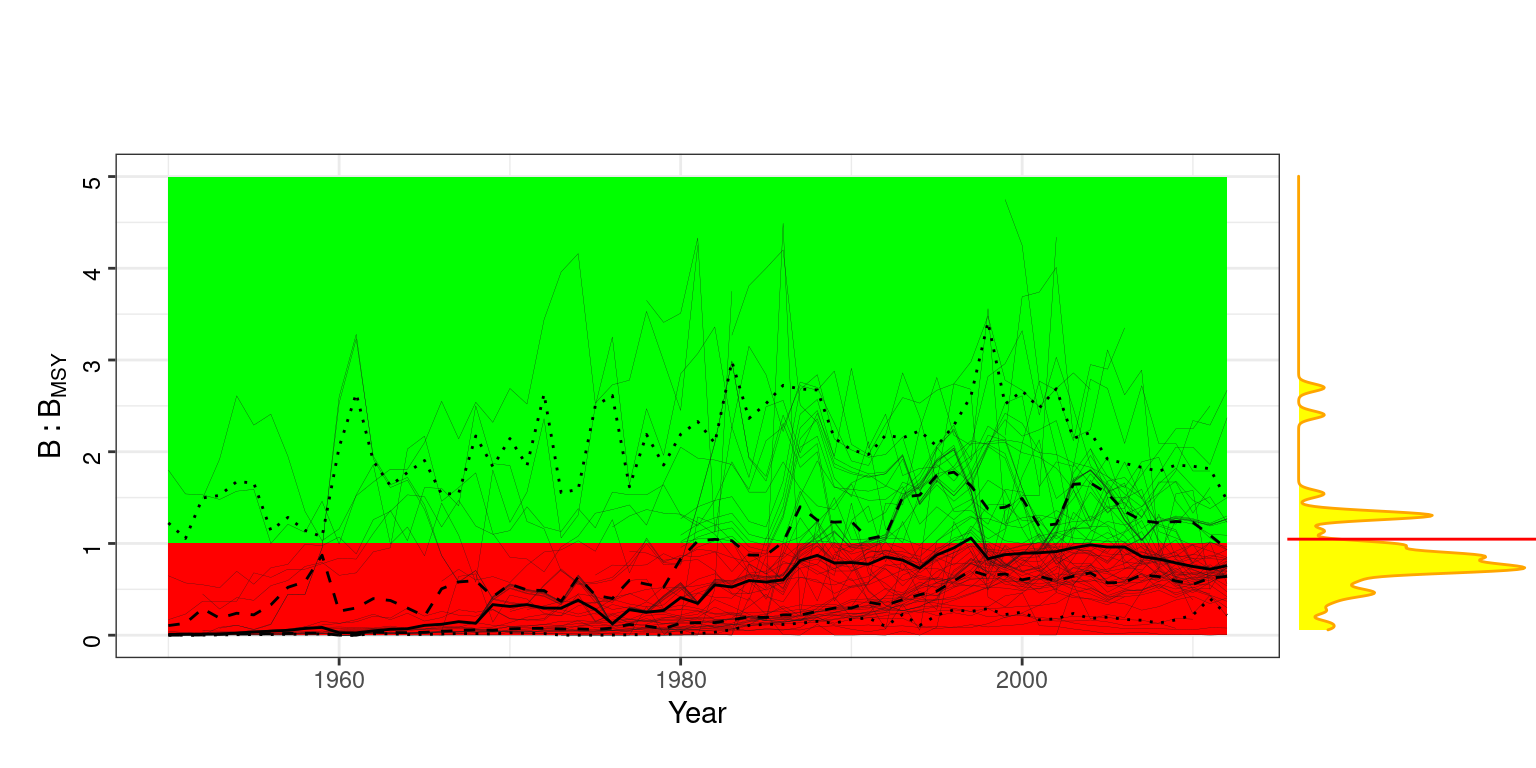
\includegraphics[width=0.75\textwidth]{figs/ts-f-1.png}
\caption{Time series of $F:F_{MSY}$ for the RAM Legacy database assessments.}
\label{fig:ts-f}
\end{figure}

\begin{figure}[ht!]
\centering
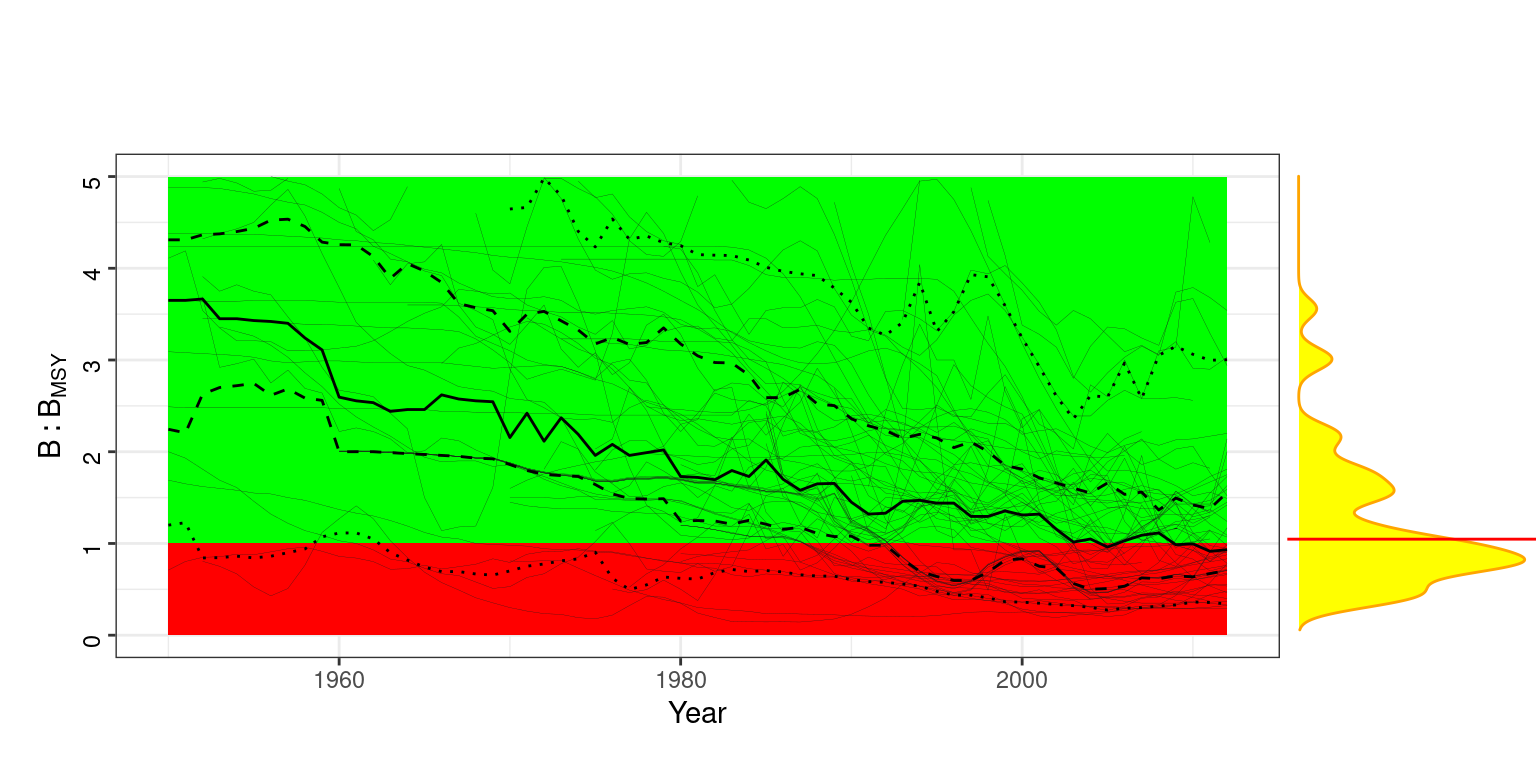
\includegraphics[width=0.75\textwidth]{figs/ts-ssb-1.png}
\caption{Time series of $B:B_{MSY}$ for the RAM Legacy database assessments.}
\label{fig:ts-s}
\end{figure}

\begin{figure}[ht!]
\centering
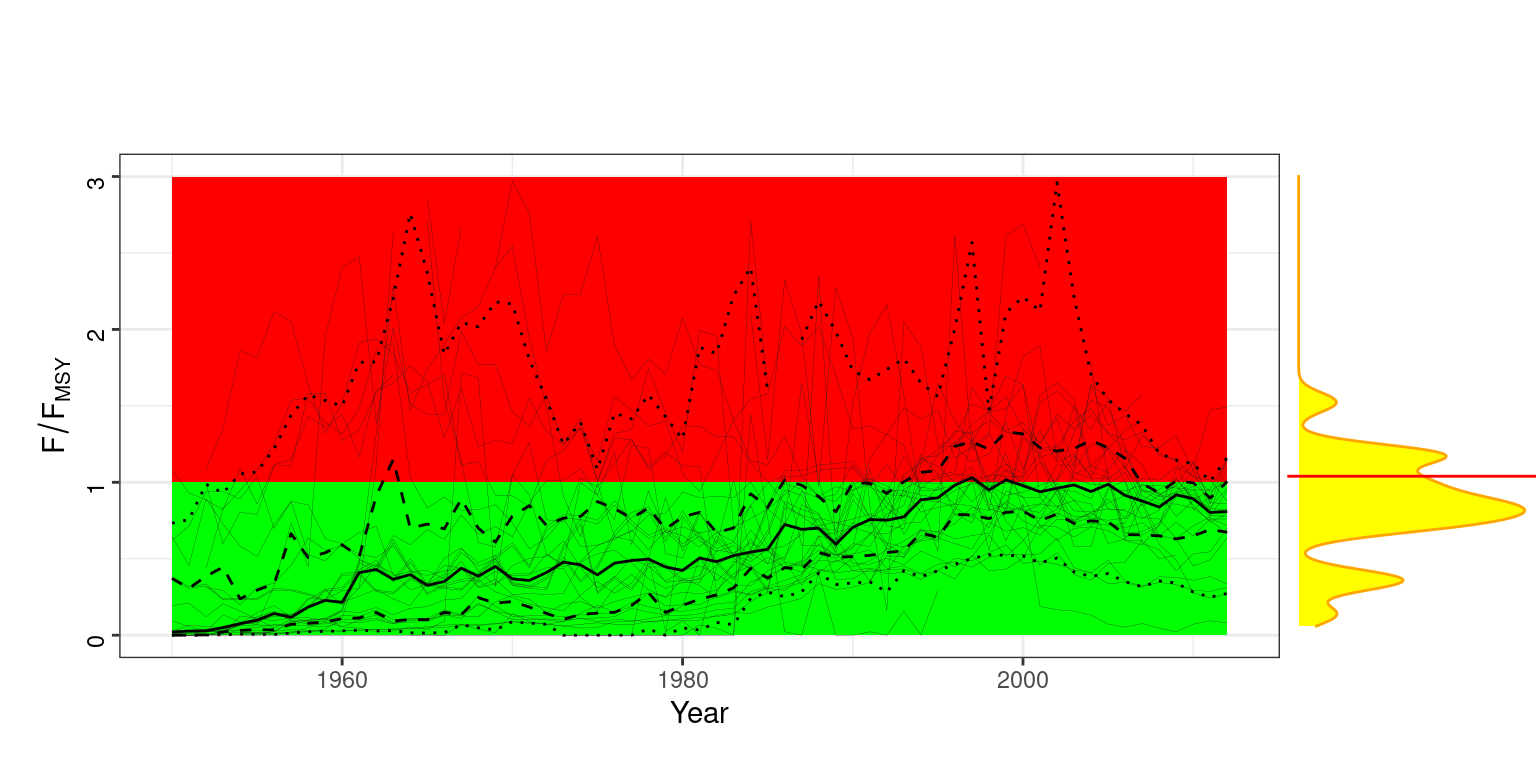
\includegraphics[width=0.75\textwidth]{figs/ts-c-1.png}
\caption{Time series of $Catch:MSY$ for the RAM Legacy database assessments.}
\label{fig:ts-c}
\end{figure}

\begin{figure}[ht!]
\centering
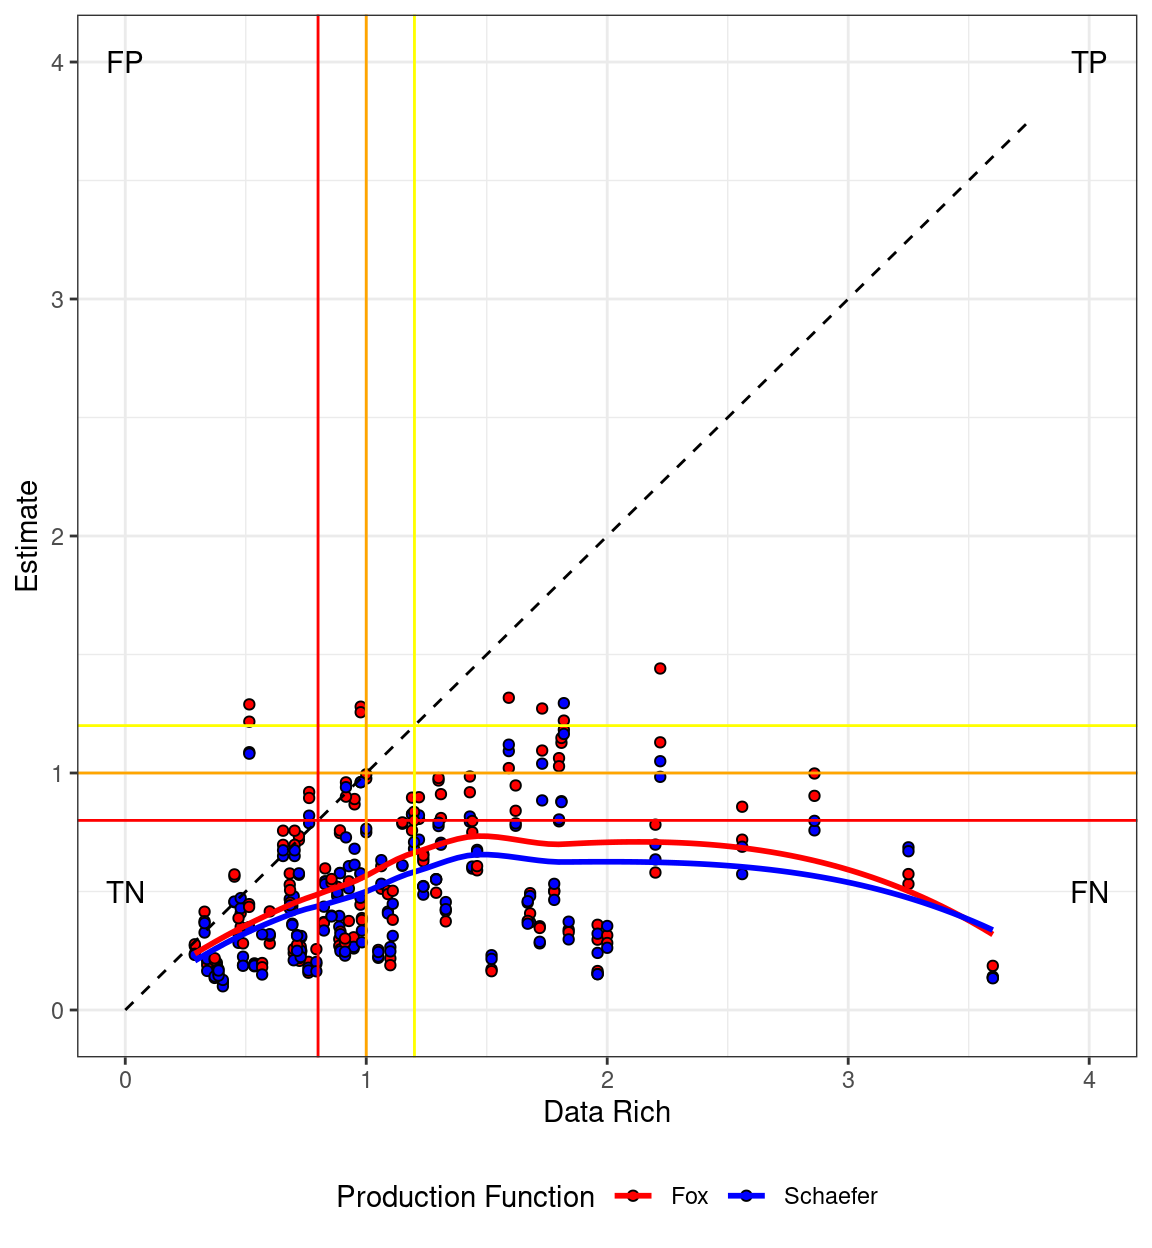
\includegraphics[width=0.75\textwidth]{figs/cf-jabba-1.png}
\caption{Comparisons of $B:B_{MSY}$, If the COM was unbiased y=x, if COM was biased but tunable then the smoother should be linear.}
\label{fig:cf-com}
\end{figure}

\begin{figure}[ht!]
\centering
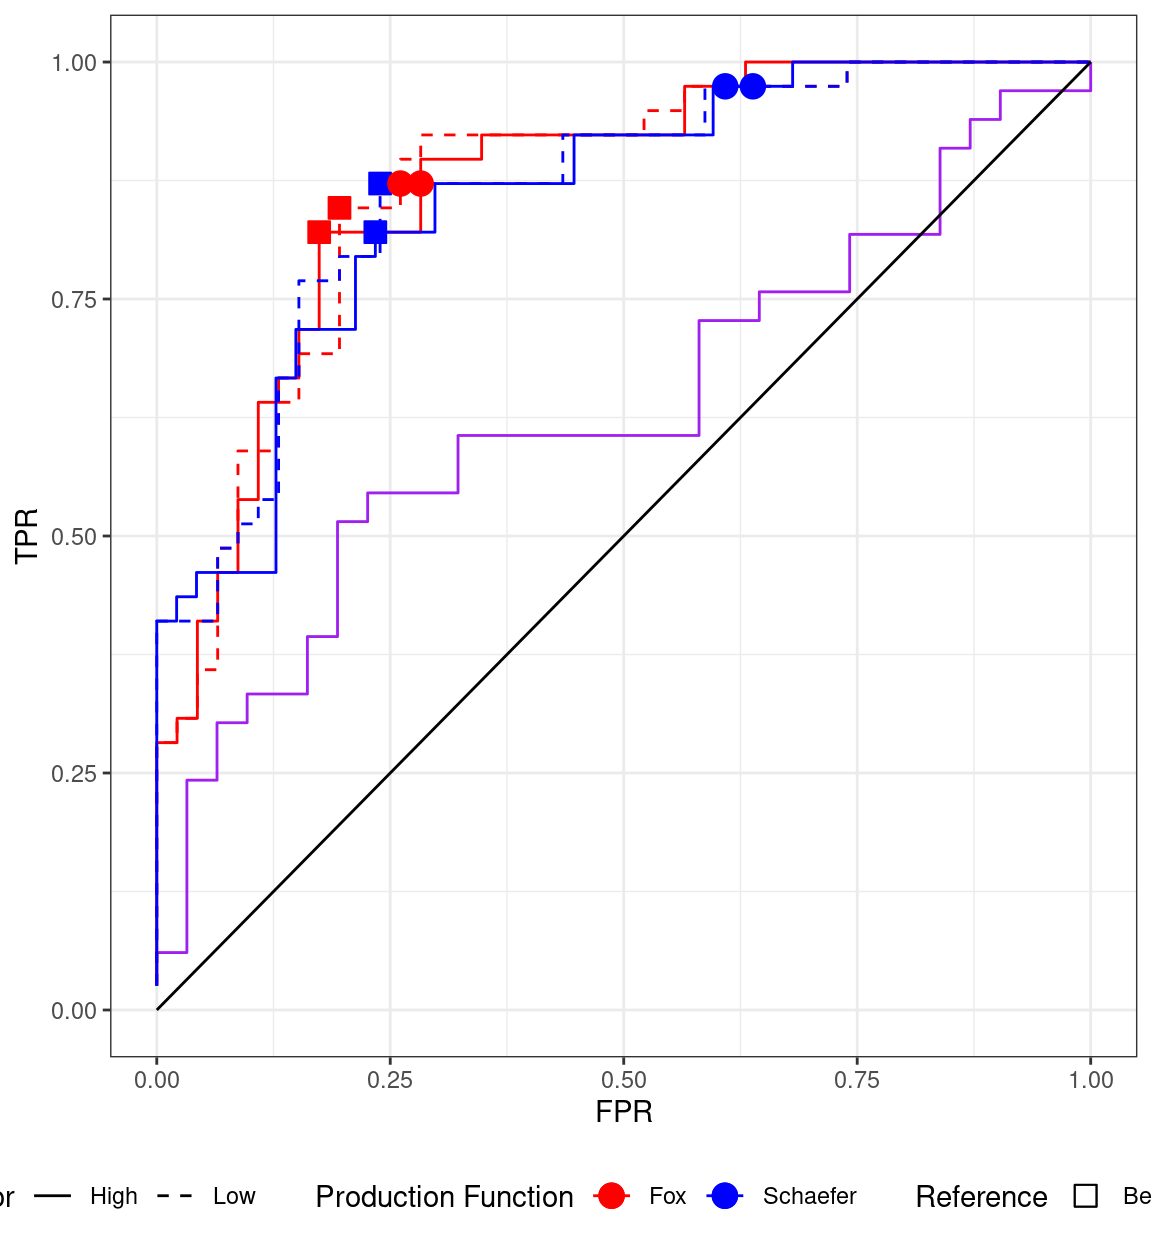
\includegraphics[width=0.75\textwidth]{figs/roc-jabba-1.png}
\caption{ROC curves for COMs.}
\label{fig:roc-com}
\end{figure}

\begin{figure}[ht!]
\centering
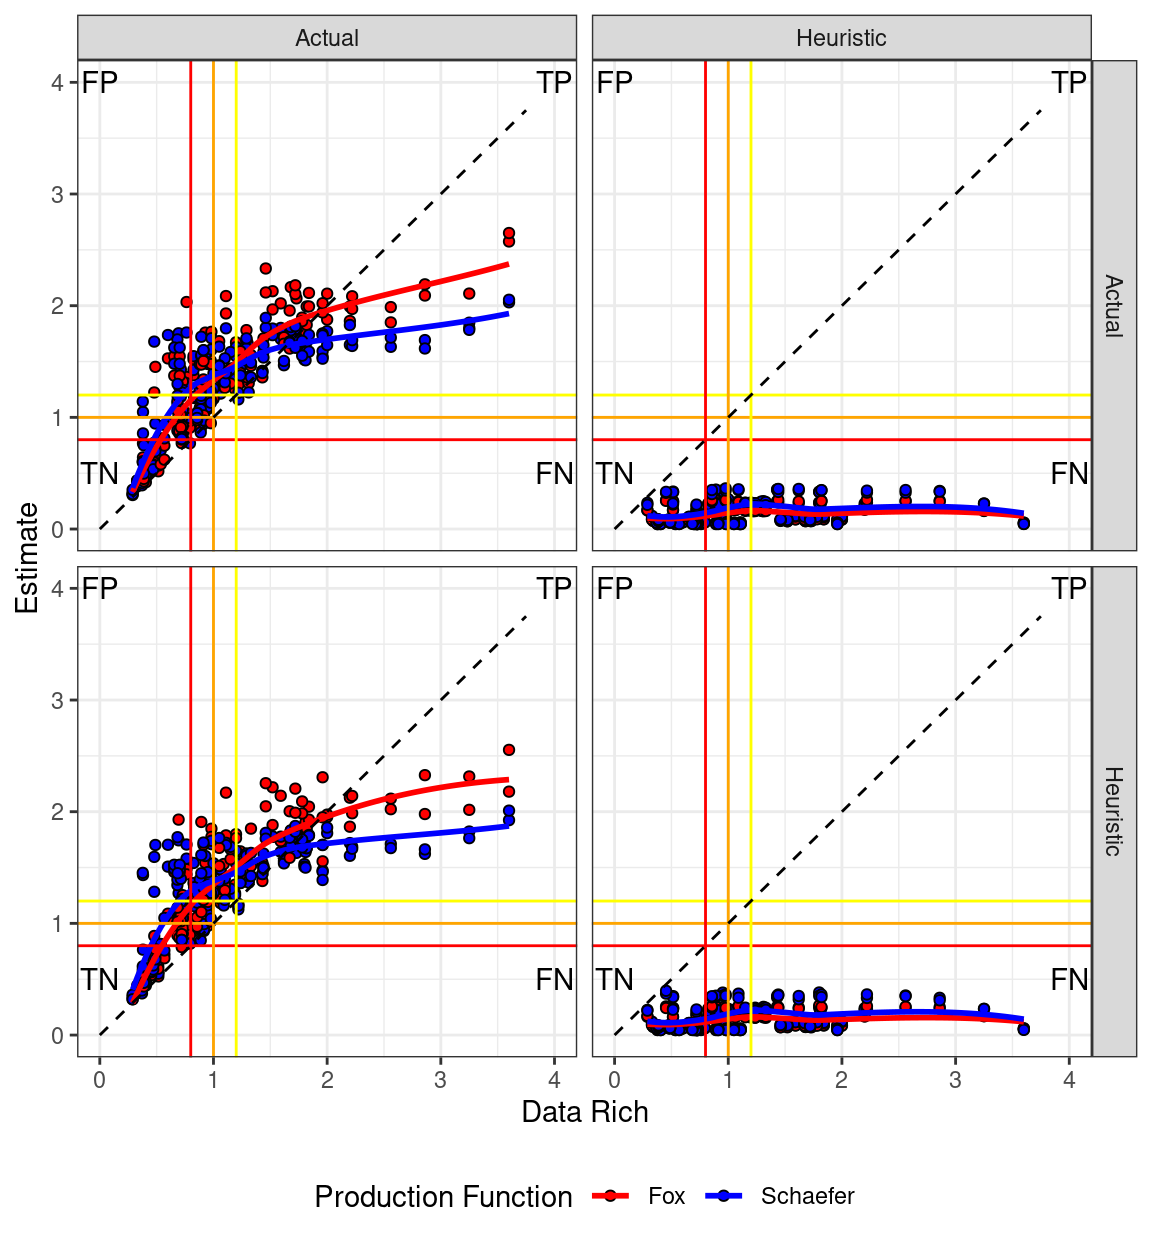
\includegraphics[width=0.75\textwidth]{figs/cf-1.png}
\caption{Comparisons of $B:B_{MSY}$, If the COM was unbiased y=x, if COM was biased but tunable then the smoother should be linear.}
\label{fig:cf}
\end{figure}

\begin{figure}[ht!]
\centering
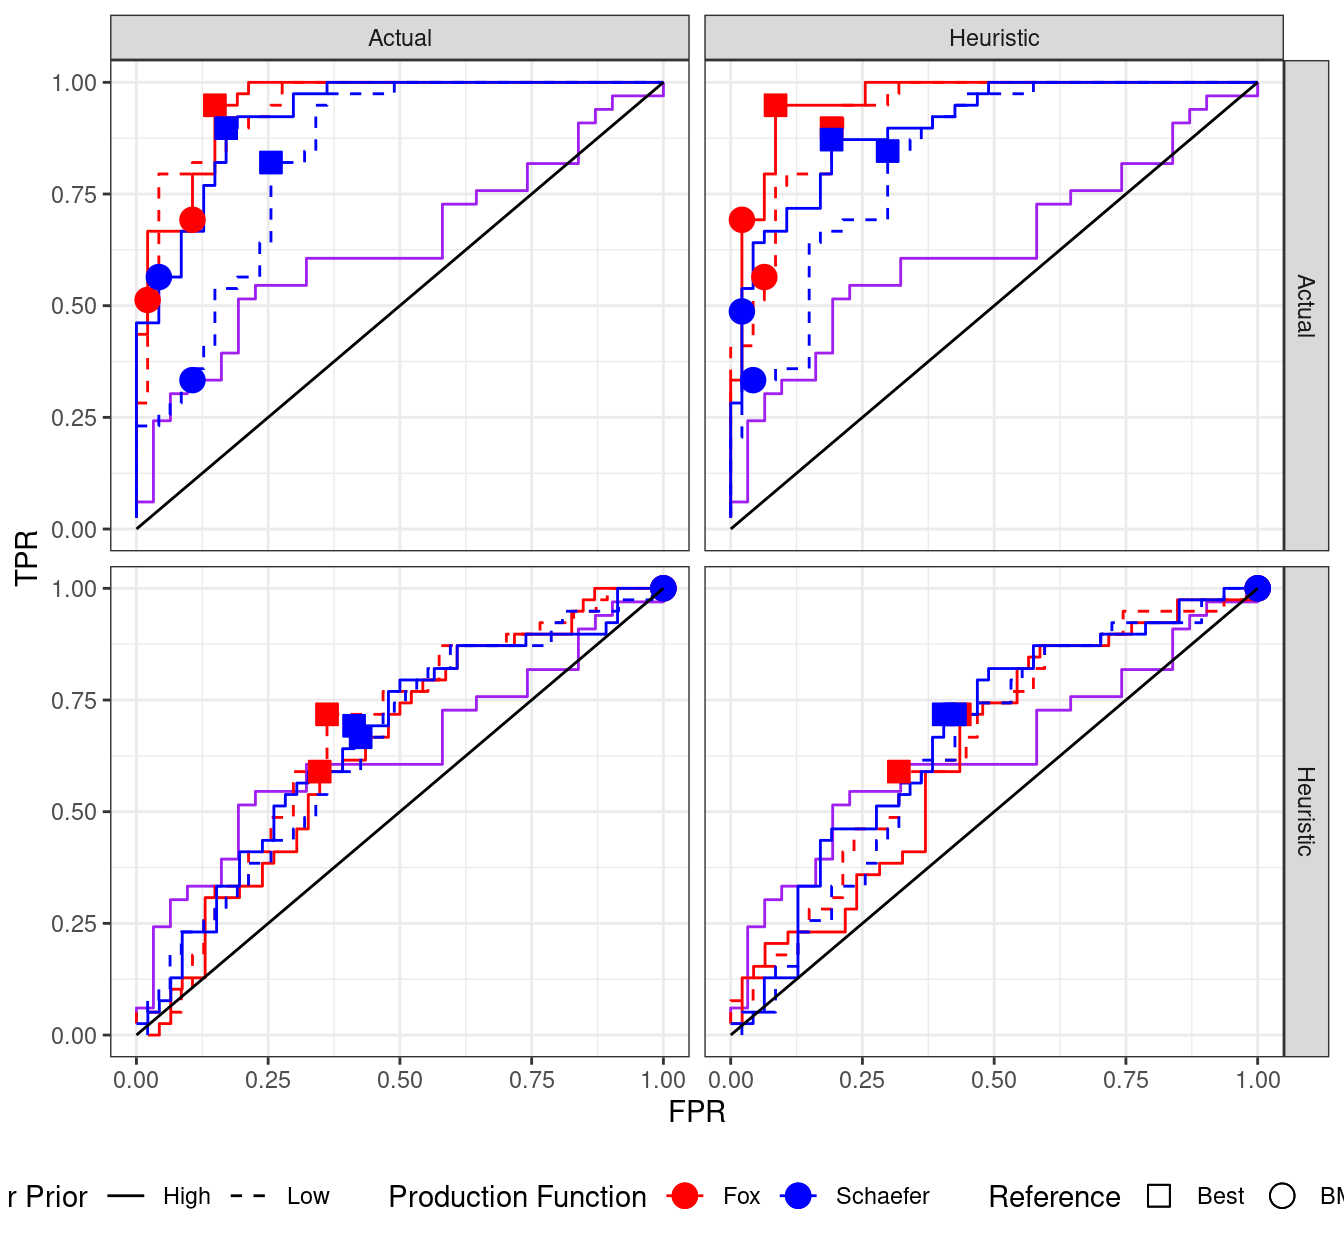
\includegraphics[width=0.75\textwidth]{figs/roc-1.png}
\caption{ROC curves for COMs.}
\label{fig:roc}
\end{figure}


\newpage
\clearpage\newpage
\section*{Supplementary Material}
%\begin{figure}[ht!]
\centering
\includegraphics[width=0.75\textwidth]{figs/ts-hh-1.png}
\caption{Time series of $B:B_{MSY}$ by stock for the RAM Legacy database assessments.}
\label{fig:ts}
\end{figure}

\begin{figure}[ht!]
\centering
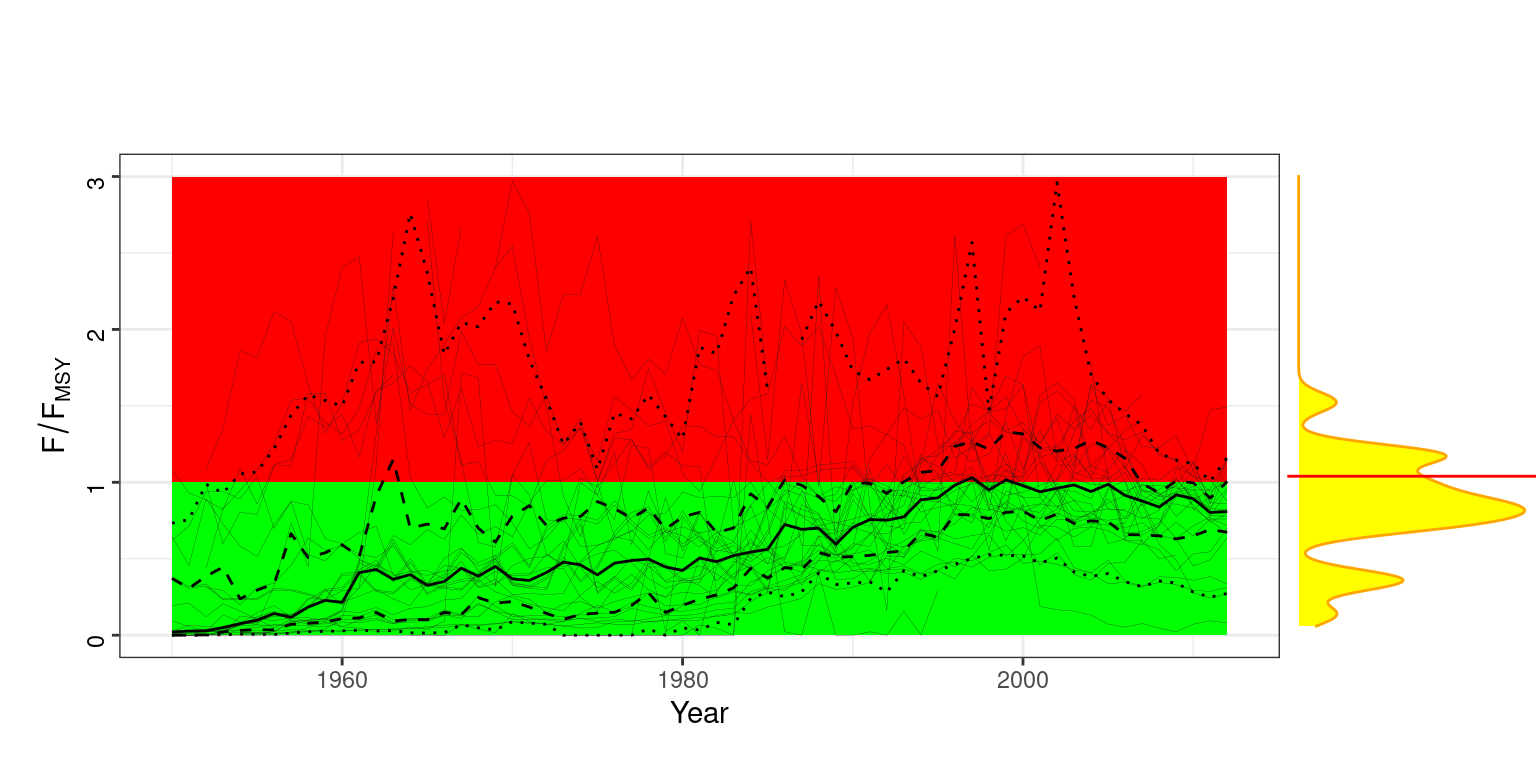
\includegraphics[width=0.75\textwidth]{figs/ts-c-1.png}
\caption{Time series of $Catch:MSY$ for the RAM Legacy database assessments.}
\label{fig:ts-c}
\end{figure}


\begin{figure}[ht!]
\centering
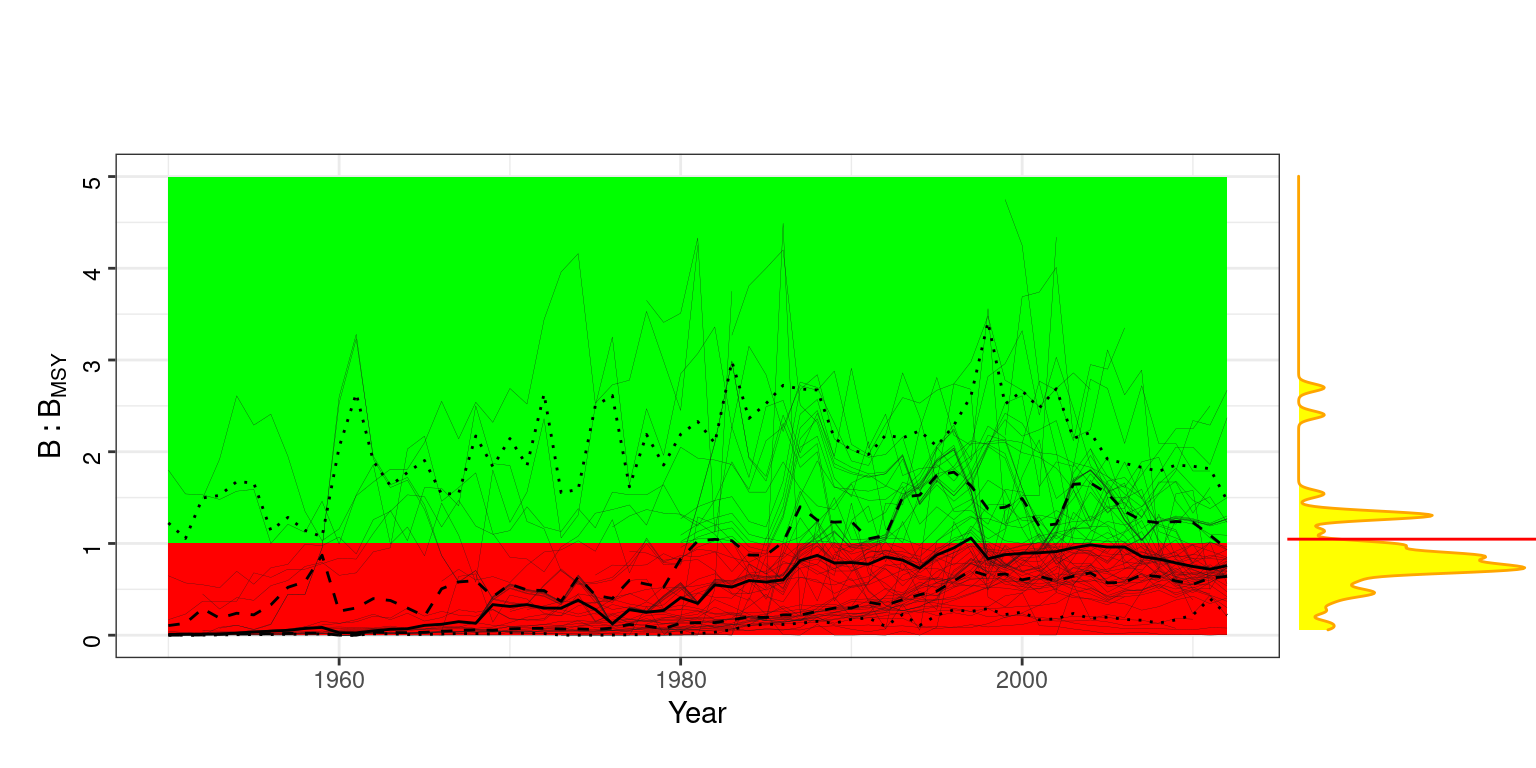
\includegraphics[width=0.75\textwidth]{figs/ts-f-1.png}
\caption{Time series of $F:F_{MSY}$ for the RAM Legacy database assessments.}
\label{fig:ts-f}
\end{figure}

\begin{figure}[ht!]
\centering
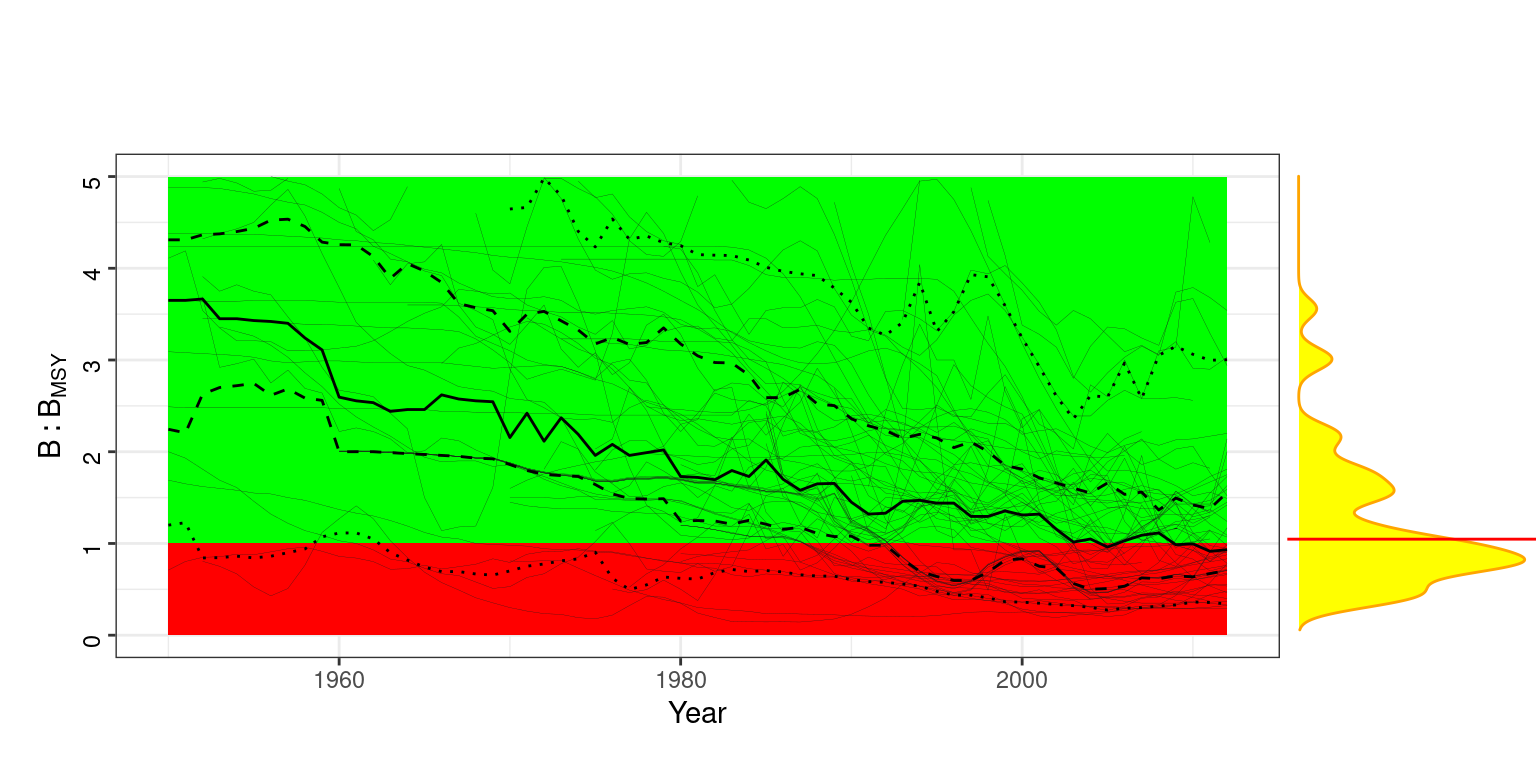
\includegraphics[width=0.75\textwidth]{figs/ts-ssb-1.png}
\caption{Time series of $B:B_{MSY}$ for the RAM Legacy database assessments.}
\label{fig:ts-s}
\end{figure}


\begin{figure}[ht!]
\centering
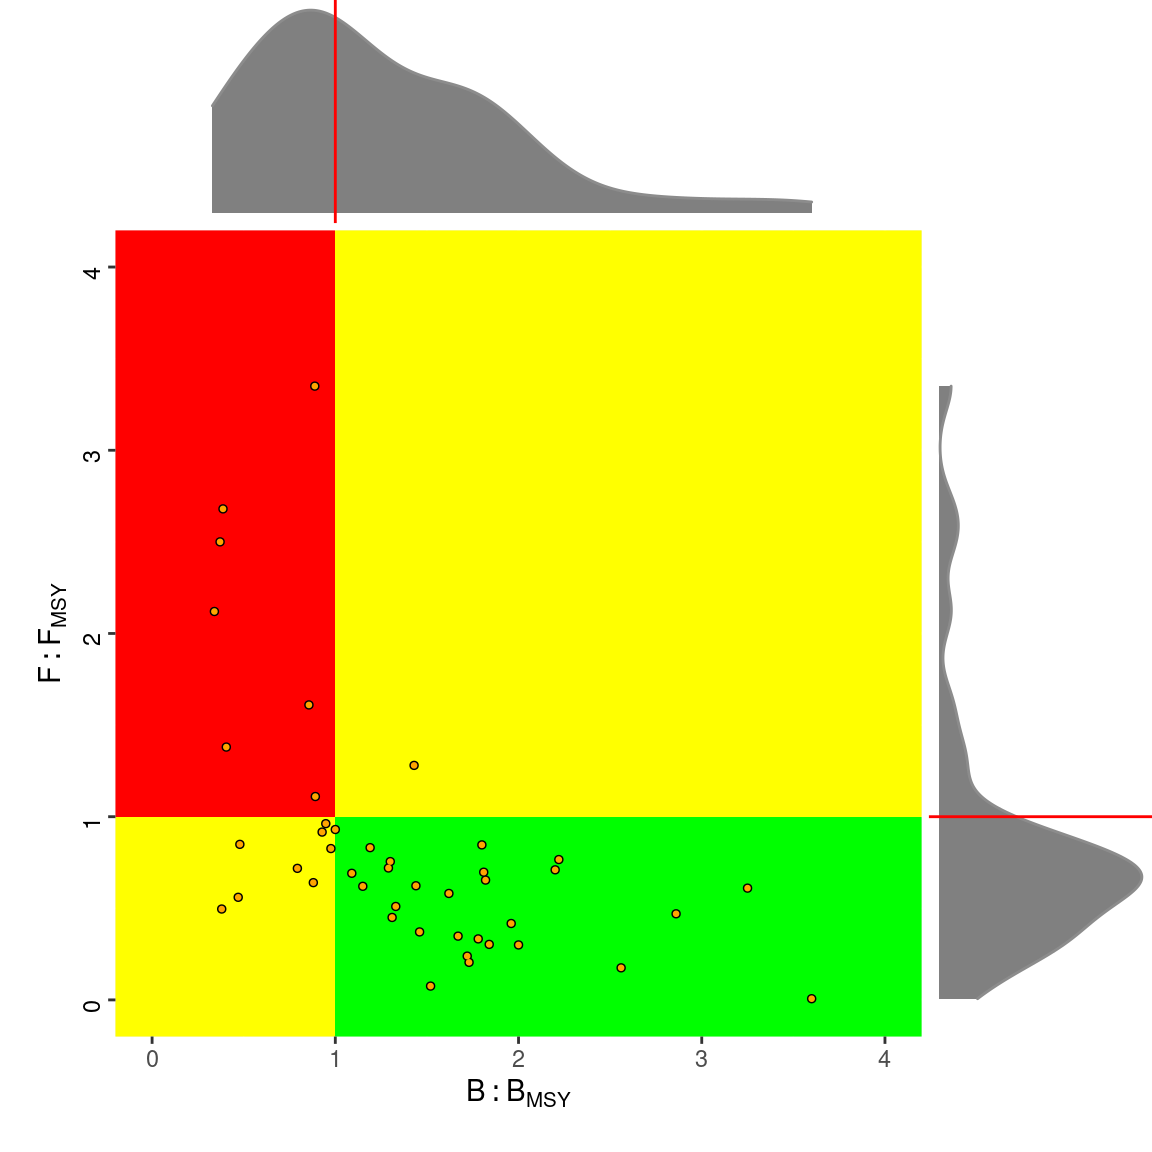
\includegraphics[width=0.75\textwidth]{figs/kobe-1.png}
\caption{Kobe phase plot.}
\label{fig:kobe}
\end{figure}

\begin{figure}[ht!]
\centering
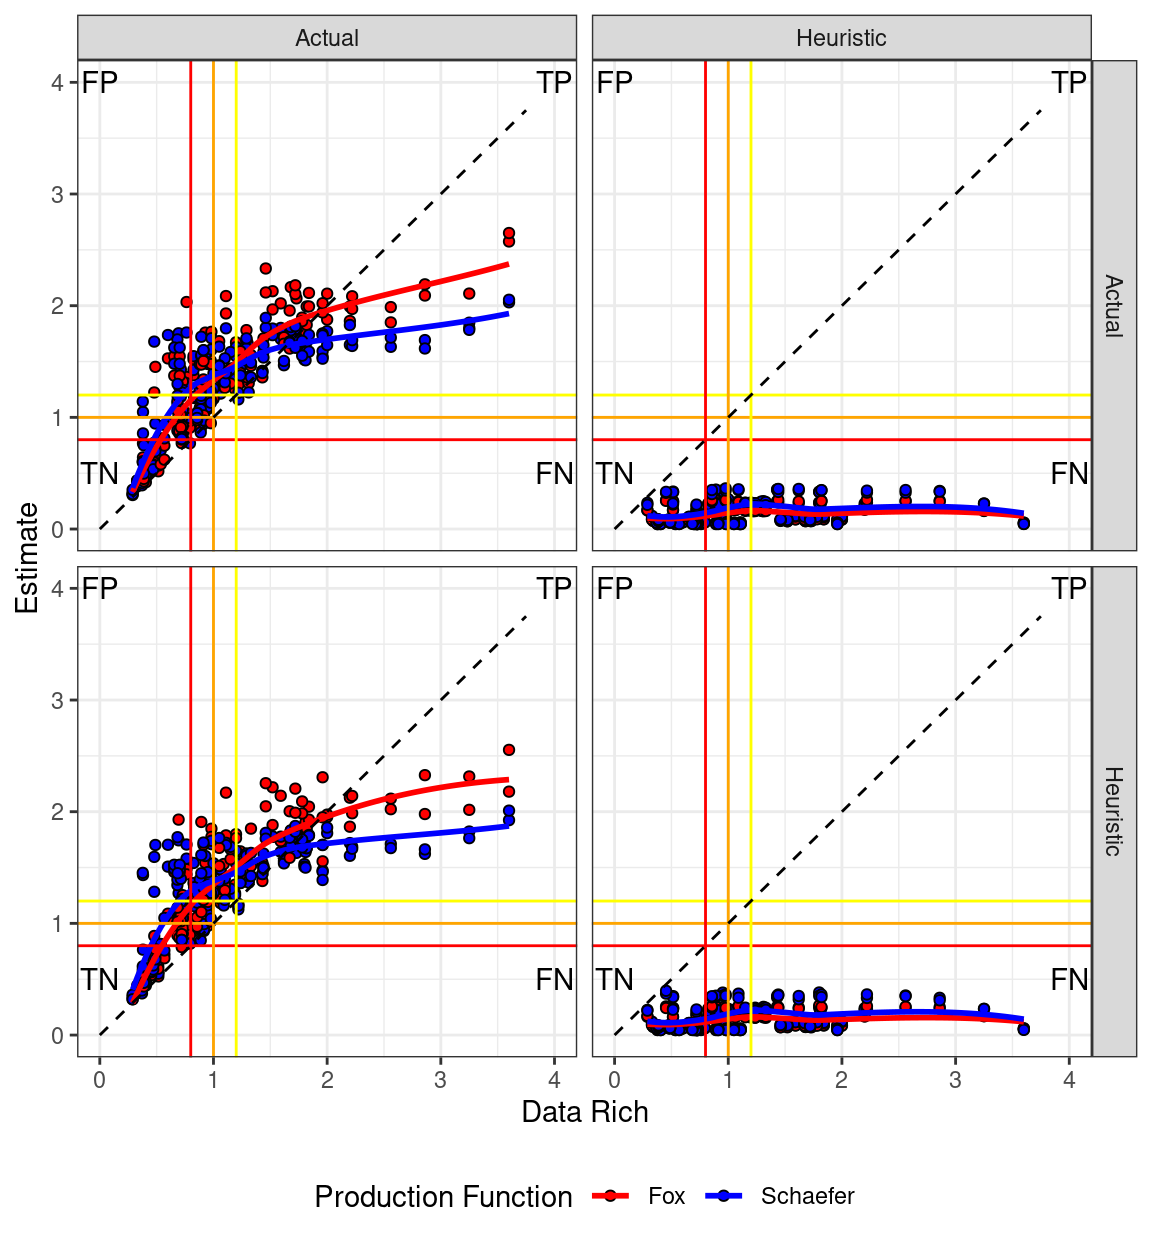
\includegraphics[width=0.75\textwidth]{figs/cf-1.png}
\caption{Comparisons of $B:B_{MSY}$.}
\label{fig:cf}
\end{figure}

\begin{figure}[ht!]
\centering
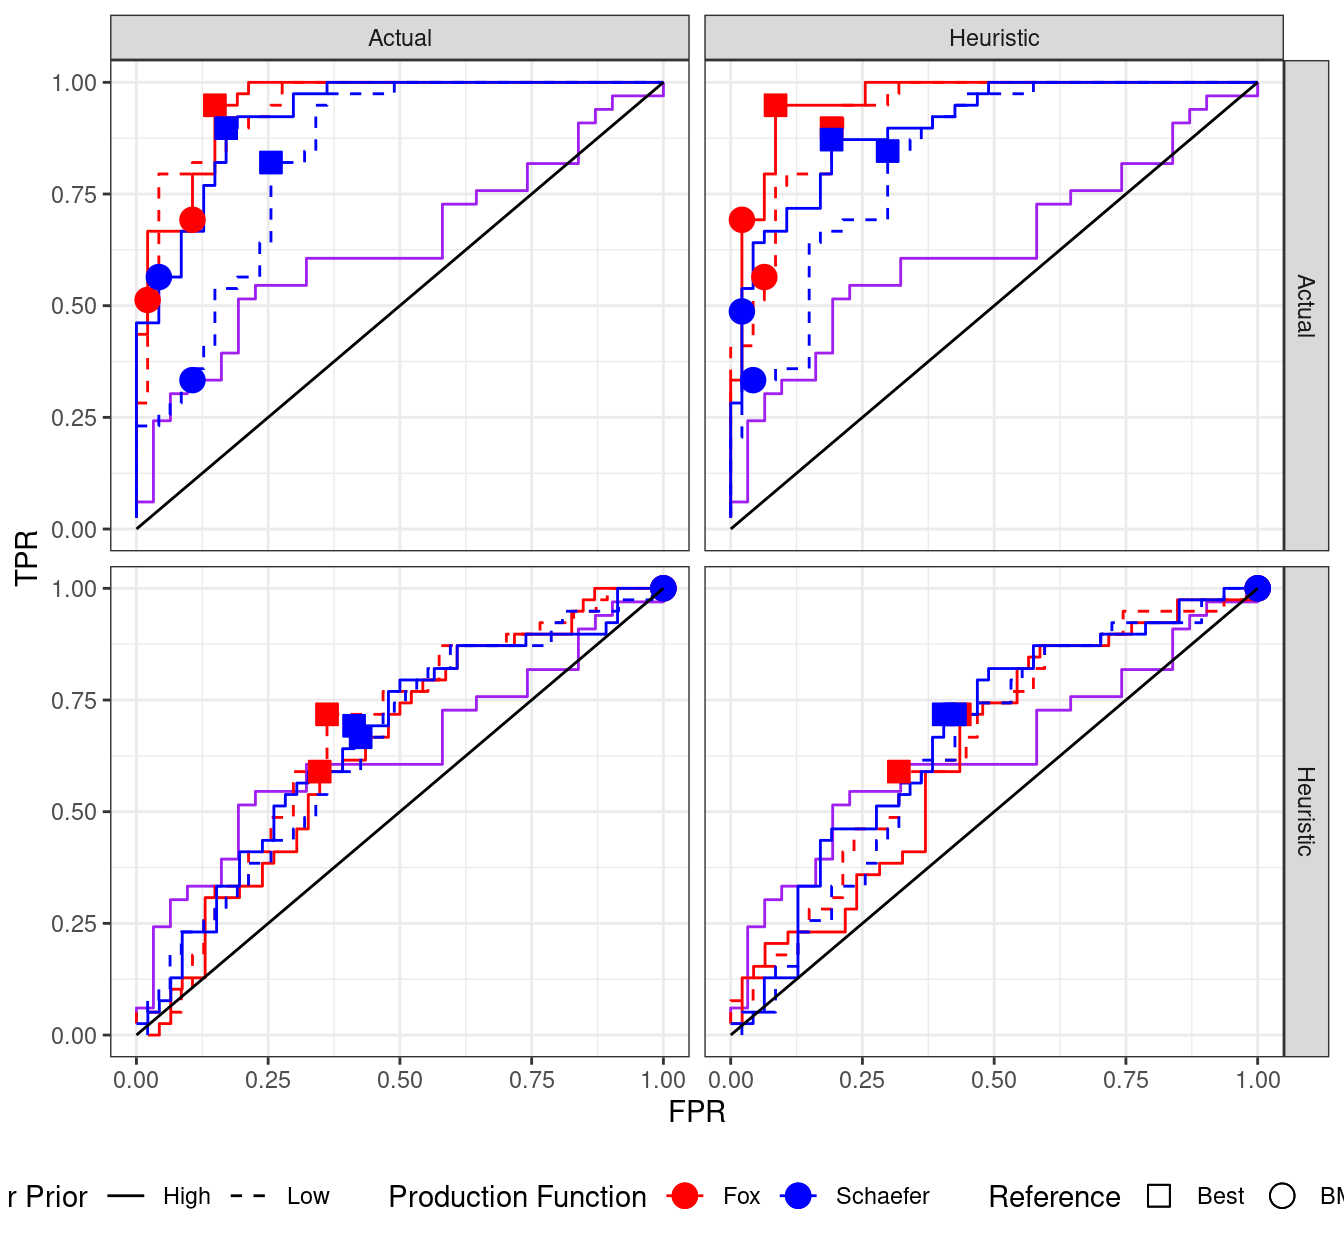
\includegraphics[width=0.75\textwidth]{figs/roc-1.png}
\caption{ROC curves for COMs.}
\label{fig:roc}
\end{figure}


\begin{figure}[ht!]
\centering
\includegraphics[width=0.75\textwidth]{figs/roc-index-1.png}
\caption{ROC curve for JABBA fitted to perfect index.}
\label{fig:roc-index}
\end{figure}





\end{document}
